\section{A Technical Tool to Quantify the Bias-Variance Trade-off}
\label{sec_main}

We revisit the classical bias-variance trade-off in the context of multi-task learning for linear regressions, in particular the setup of equation \eqref{eq_mtl}.
For the high-dimensional setting where the data size of the target task is a small constant times dimension $p$, we quantify the trade-off as a function of the task models $\set{\beta_i}_{i=1}^t$, data size $\set{n_i}_{i=1}^t$, and covariance matrices $\set{\Sigma_i}_{i=1}^t$.

\textbf{Multi-task learning.} Our first result applies to the setting of two tasks where their covariance matrices may be arbitrarily different.
%The technical crux of our approach is to derive the asymptotic limit of $\te(\hat{\beta}_t^{\MTL})$ in the high-dimensional setting, when $p$ approaches infinity.
We derive a precise limit of $\bigtr{(X_1^{\top}X_1 + X_2^{\top}X_2)^{-1}\Sigma_2}$, which is a deterministic function that only depends on $\Sigma_1, \Sigma_2$ and $n_1/p, n_2/p$ (see Lemma \ref{lem_cov_shift} in Appendix \ref{app_proof_main} for the result).
Based on the result, we show how to determine positive versus negative transfer as follows.

\begin{theorem}[Informal]\label{thm_main_informal}
	Let $X_i \in\real^{n_i \times p}$ and $Y_i = X_i\beta_i + \varepsilon_i$, for $i = 1, 2$.
	Suppose that $n_1 = \rho_1 p$ and $n_2 = \rho_2 p$, where $\rho_1>1$ and $\rho_2 >1$ are fixed constants.
	There exists two deterministic functions $\Delta_{\beta}$ and $\Delta_{\vari}$ and a small deterministic error $\delta$ that only depend on $\set{\hat{v}, \Sigma_1^{}, n_1, n_2, \beta_1, \beta_2}$ such that
	\begin{itemize}
		\item If $\Delta_{\vari} - \Delta_{\beta} \ge \delta$, then whp $\te(\hat{\beta}_t^{\MTL}) < \te(\hat{\beta}_t^{\STL})$.
		\item If $\Delta_{\vari} - \Delta_{\beta} \le \delta$, then whp $\te(\hat{\beta}_t^{\MTL}) > \te(\hat{\beta}_t^{\STL})$.
	\end{itemize}
\end{theorem}

Theorem \ref{thm_main_informal} shows nearly tight bounds on the trade-off between model-shift bias and variance reduction.
%determined by the covariate shift matrix and the model shift.
The bounds get tighter and tighter as $\rho_1$ increases.
A formal version of Theorem \ref{thm_main_informal} is presented in Theorem \ref{thm_model_shift} and its proof is presented in Appendix \ref{app_proof_main}.
While the general form of $\Delta_{\vari}$ and $\Delta_{\beta}$ can be quite complex, we show that they provide nice interpretation for several simple settings in the rest of the section.

\textit{Proof overview.} By comparing the bias and variance of $\te_t(\hat{\beta}_t^{\MTL})$ to $\te_t(\hat{\beta}_t^{\STL})$, we observe the following two effects, respectively.
%We begin by observing that the test error of $\hat{\beta}_t^{\MTL}$ consists of two parts.
We term equation \eqref{eq_te_model_shift} as \textit{model-shift bias}, which captures how similar $\beta_1$ and $\beta_2$ are.
This part introduces a negative effect to multi-task learning.
The scaling term $\hat{v}$ corresponds to the intuition that the shared module $B$ learns a subspace for both tasks.
The output layer of each task scales the direction of $B$ suitably to fit the task.

Next, it is not hard to verify that equation \eqref{eq_te_var}, the variance of $\hat{\beta}_t^{\MTL}$, is always smaller than the variance of $\hat{\beta}_t^{\STL}$.
This part introduces a positive variance reduction effect to performing multi-task learning.
Hence, whether $\te(\hat{\beta}_t^{\MTL})$ is lower than $\te(\hat{\beta}_t^{\STL})$ is determined by the trade-off between two effects:
(i) the positive effect from variance reduction;
(ii) the negative effect from model shift bias.

Our second result applies to the setting of any number of tasks with the same covariates.
%We extend the above result to any number of tasks that have the same covariates.
%In this section we consider the setting with $k$ many that have the same covariates.
Since the tasks all have the same number of datapoints and covariance matrix, the trade-off between model shift bias and variance will be captured by their task models $\set{\beta_i}_{i=1}^k$.
%For this setting, we derive solutions for the multi-task training and the transfer learning setting that match our insights qualitatively from Section \ref{sec_denoise}.
Let $B^{\star} = [\beta_1, \beta_2, \dots, \beta_k] \in\real^{p\times k}$ denote the underlying task model parameters.
We can also derive a tight trade-off between model shift bias and variance reduction for this setting.
The formal statement is stated in Theorem \ref{thm_many_tasks} and its proof can be found in Appendix \ref{app_proof_many_tasks}.

\textbf{Extensions to transfer learning.}
While our focus is on multi-task learning, we show that our results extend to transfer learning settings naturally.
We provide an analysis of the transfer function of Taskonomy \cite{ZSSGM18} using our setup.
Specifically, the source task encoder consists of the representations learnt from one or more source tasks.
The transfer function then tries to fit the target task data to the source task encoder.
For more details, we refer the reader to Figure 4 in Taskonomy.

We map the procedure to our setup as follows.
First, we obtain the single-task estimator $\hat{\beta}_i$ from the source tasks, for $1\le i \le t-1$.
This forms the shared representation $B^{\star}_{t-1} = [\hat{\beta}_1,\hat{\beta}_2,\dots,\hat{\beta}_{t-1}]$.
Then, we learn the output layer $W_t$ on the target task by minimizing the following objective
\begin{align}
	g(W_t) = \bignorm{X_t B W_t - Y_t}^2.
\end{align}
After solving $W_t$, we use $\hat{\beta}_t^{\TL} = B W_t$ as the estimator for the target task.
By comparing $\te(\hat{\beta}_t^{\TL})$ to $\te(\hat{\beta}_t^{\STL})$, we observe a similar trade-off between model-shift bias and variance reduction for this setting.
%We use our tools to compare $\te(B W_t)$ to $\te(\beta_t^{\STL})$.
The formal statement is presented in Theorem \ref{prop_taskonomy} and its proof in Appendix \ref{app_proof_sec4}.





\section{Theoretical Implications}
\label{sec_insight}

After describing this technical result, we provide theoretical insights over when multi-task learning performs better than single-task learning.
Our analysis reveals three contributing causes of negative transfer, including task model \textit{dissimilarity}, \textit{unbalanced} data size, and \textit{covariate shift}, which we describe in detail for the rest of the section.


\subsection{Contributing causes of negative transfer}

A folklore intuition since the seminal work of Caruana \cite{C97} is that task relatedness determines how well multi-task learning performs.
We formalize the intuition using our setup and technical tools.

\textbf{Task model dissimilarity.}
For a simple example of two tasks, we show that whether $\hat{\beta}_t^{\MTL} \le \hat{\beta}_t^{\STL}$ is determined by $\norm{\beta_1 - \beta_2}^2$, the distance of the task models.
We derive a sharp threshold when positive transfer transitions to negative transfer, as a function of model distance $\norm{\beta_1 - \beta_2}^2$, data size $n_1$ abd $n_2$ and the noise level $\sigma$.

\textit{A simplifying setting.}\label{ex_basic}
	Consider a setting where $\Sigma_1 = \Sigma_2 = \id$, in other words there is no covariate shift between the two tasks. For the noises, we assume that $\e_i$ has i.i.d. entries with mean zero and variances $\sigma_i^2$, $i=1,2$.
	For the task models, suppose that $\beta_2$ has i.i.d. entries with mean zero and variance $\kappa^2$ and $\beta_1 - \beta_2$ also has i.i.d. entries with mean $0$ and variance $d^2$.
	%The noise level for both tasks is equal to $\sigma > 0$.
	We have $n_i = \rho_i \cdot p$ data points from each task, for $i = 1, 2$.
	For simplicity, we assume that all the random variables have subexponential decay, while keeping in mind that our results can be applied under weaker moments assumptions as shown in the supplementary material.

We illustrate the example with a simulation.
We consider a setting where $p = 200$, $n_1 = 90p$, $n_2 = 30p$.
We fix the target task and vary the source task, in particular the parameter $d$ which determines $\norm{\beta_1 - \beta_2}$.
Figure \ref{fig_model_shift} shows the result.
Based on Theorem \ref{thm_model_shift}, we derive the transition threshold in the following proposition.
Define the following function
\begin{align*}
	\Phi(\rho_1, \rho_2) = \frac{(\rho_1 + \rho_2 - 1)^2}{\rho_1 (\rho_1 + \rho_2) (\rho_2 - 1)}.
\end{align*}

\begin{proposition}\label{prop_dist_transition}
	In the simplifying setting with $\sigma_1 = \sigma_2 = \sigma$, assume that $\rho_1 > 40$ is a fixed constant.
	Whether $\te(\hat{\beta}_t^{\MTL})$ is lower than $\te(\hat{\beta}_t^{\STL})$ is determined by the ratio between the model distance and the noise level:
	\begin{itemize}
		\item If ${d^2} < \frac {\sigma^2} {2p} \cdot \Phi(\rho_1, \rho_2)$, then whp we have that $\te(\hat{\beta}_t^{\MTL}) < \te(\hat{\beta}_t^{\STL})$.
		\item If ${d^2} \ge \frac {2\sigma^2} {p} \cdot \Phi(\rho_1, \rho_2)$, then whp we have that $\te(\hat{\beta}_t^{\MTL}) \ge \te(\hat{\beta}_t^{\STL})$.
	\end{itemize}
\end{proposition}

We remark that the constants $1/2$ and $2$ in the statement above are chosen for the simplicity of presentation.
In general we can close the gap between the two constants by increasing $\rho_1$.
While the statement of Theorem \ref{thm_main_informal} only applies to the asymptotic regime of $p$ going to infinity, Proposition \ref{prop_dist_transition} explains most of the observations in Figure \ref{fig_model_shift} when $p = 200$.
%in this proposition (and the following ones) can be replaced with $(1+c_1^{-1/2})^{-4}$ and $(1-c_1^{-1/2})^{-4}$. In particular, these bounds becomes tighter as $c_1$ increases.

The proof of Proposition \ref{prop_dist_transition} involves two parts.
First, in equation \eqref{eq_te_var}, the positive variance reduction effect scales with $n_1 = \rho_1 p$, the number of source task data points.
Second, we show that the negative effect of model-shift bias scales with $pd^2$, which is the expectation of $\norm{\beta_1 - \beta_2}^2$.
The proof, which is based on Theorem \ref{thm_main_informal}, can be found in Appendix \ref{app_proof_31}. %, which is based on our main result described later in Theorem \ref{thm_model_shift}.

\begin{figure}
	\begin{subfigure}[b]{0.32\textwidth}
		\centering
		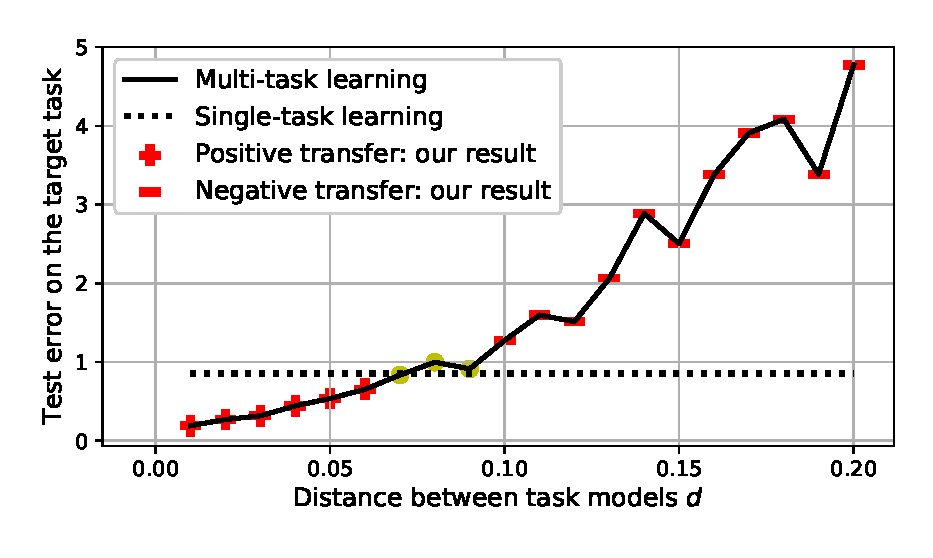
\includegraphics[width=0.98\textwidth]{figures/model_shift_phase_transition.eps}
		\caption{Task model similarity}
		\label{fig_model_shift}
	\end{subfigure}\hfill
	\begin{subfigure}[b]{0.32\textwidth}
		\centering
		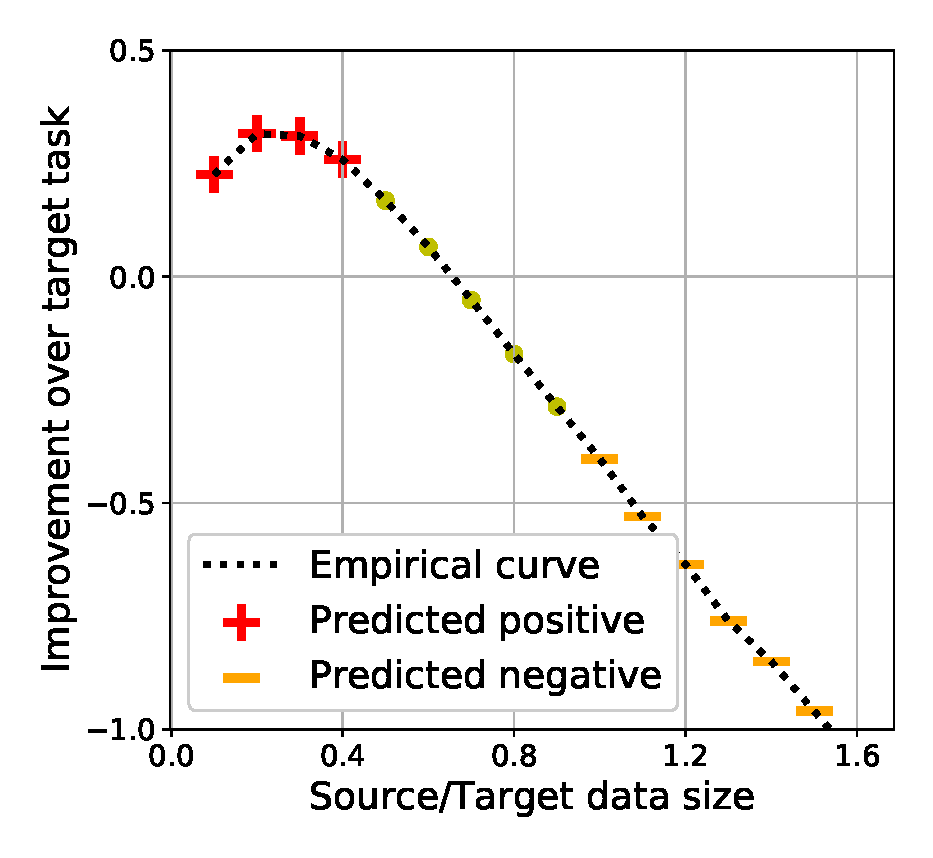
\includegraphics[width=0.98\textwidth]{figures/datapoints_phase_transition.eps}
		\caption{Data size}
	\end{subfigure}\hfill
	\begin{subfigure}[b]{0.32\textwidth}
		\centering
		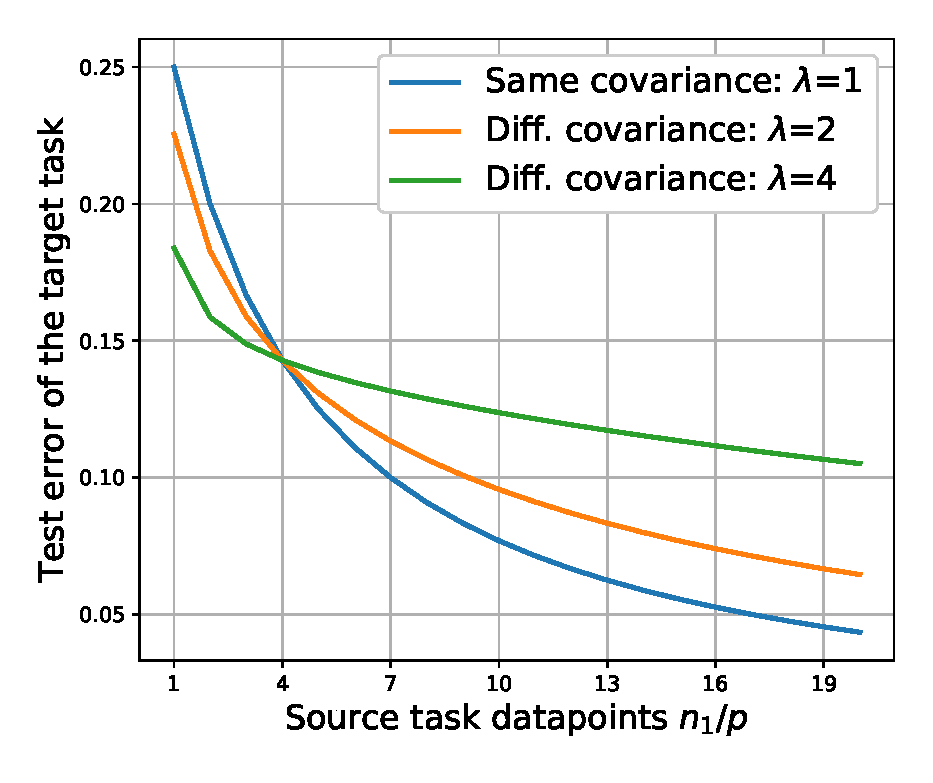
\includegraphics[width=0.98\textwidth]{figures/complementary.eps}
		\caption{Covariate shift}
		\label{fig_covariate}
	\end{subfigure}
	\caption{Comparing the test error of multi-task learning to single-task learning: (a) positive to negative transfer as the task model dissimilarity increases (cf. Proposition \ref{prop_dist_transition}) (b) positive to negative transfer as the source task data size increases (cf. Proposition \ref{prop_data_size}); (c) }
	\label{fig_model_shift_phasetrans}
\end{figure}

\textbf{Implications.}
We further show that multi-task learning is particular powerful when the labeled data of the source task is less noisy compared to the target task.
Consider a more general setting of Proposition \ref{prop_dist_transition} where the noise level $\sigma_1$ of task $1$ differs from the noise level $\sigma_2$ of task $2$.
We derive a sharp transition from positive to negative transfer as a parameter of $\sigma_1^2$.

\begin{proposition}\label{prop_var_transition}
	In the setting of Example \ref{ex_basic} with $d$ being fixed but $\sigma_1$ varies, assume that $\rho_1 > 50$ is a fixed constant and $d^2 < \frac {\sigma_2^2} {2p} \cdot \Phi(\rho_1, \rho_2)$.
	We derive the following transition as a parameter of $\sigma_1^2$:
	\begin{itemize}
		\item If $\sigma_1^2 \le -\frac32 \rho_1 \cdot p d^2+\left(1+ \frac34\rho_1 \Phi(\rho_1, \rho_2)\right)\cdot\sigma_2^2$, then whp $\te(\hat{\beta}_t^{\MTL}) < \te(\hat{\beta}_t^{\STL})$.
		\item If $\sigma_1^2 > - \frac12p d^2 \cdot \rho_1 +\left(1+ \frac32\Phi(\rho_1, \rho_2)\right) \cdot \sigma_2^2$, then whp $\te(\hat{\beta}_t^{\MTL}) > \te(\hat{\beta}_t^{\STL})$.
	\end{itemize}
\end{proposition}
As a corollary, if $\sigma_1^2 \le \sigma_2^2$, then we always get positive transfer.
The proof of Proposition \ref{prop_var_transition} is similar to Proposition \ref{prop_dist_transition}.
The details can be found in Appendix \ref{app_proof_31}.


\subsection{Improving Labeled Data Efficiency}\label{sec_data_size}

\textbf{Data size.}
In classical Rademacher or VC based theory of multi-task learning, adding more labeled data improves the generalization performance of a model.
On the other hand, we have observed that adding more labeled data does not always improve performance in multi-task learning.
Using Example \ref{ex_basic}, we analyze the effect of varying the source task data size.

\begin{proposition}\label{prop_data_size}
	In the setting of Example \ref{ex_basic}, assume that $\rho_1 > 40$ and $\rho_2 > 500$ are fixed constants.
	We have the following conditions to determine whether $\te(\hat{\beta}_t^{\MTL})$ is lower than $\te(\hat{\beta}_t^{\STL})$:
	\begin{itemize}
\item If $d^2 \le \frac{\sigma^2}{2p(\rho_2-1)}$, then whp $\te(\hat{\beta}_t^{\MTL}) < \te(\hat{\beta}_t^{\STL})$.

\item If $d^2 > \frac{2\sigma^2}{p (\rho_2 - 1)}$, then we have the following transition depending on $\rho_1$:
		\begin{itemize}
			\item If $\rho_1 < \frac{(\rho_2-2)\sigma^2}{(1 + {\rho_1}^{-0.5})^4(\rho_2 - 1) pd^2 - \sigma^2}$, then whp $\te(\hat{\beta}_t^{\MTL}) < \te(\hat{\beta}_t^{\STL})$.
			\item If $\rho_1 > \frac{(\rho_2-2) \sigma^2}{(1 - {\rho_1}^{-0.5})^4 (\rho_2 - 3) pd^2 - \sigma^2}$, then whp $\te(\hat{\beta}_t^{\MTL}) > \te(\hat{\beta}_t^{\STL})$.
		\end{itemize}
	\end{itemize}
\end{proposition}

The proof of Proposition \ref{prop_data_size} is similar to Proposition \ref{prop_dist_transition}.
We compare the model shift bias and the amount of reduced variance of $\hat{\beta}_t^{\MTL}$.
An intuitive interpretation of Proposition \ref{prop_data_size} is that:
i) If the two task models are sufficiently similar (as specified under the first bullet), adding the source task always provides positive transfer;
ii) Otherwise, as we increase the number of source task data points, the transfer is positive initially, but transitions to negative eventually.
We leave the proof of Proposition \ref{prop_data_size} to Appendix \ref{app_proof_data}.

\textbf{Covariate shift.}
So far we have considered settings where $\Sigma_1 = \Sigma_2$.
This setting is relevant for multi-class image classification settings, where different tasks share the same input features.
In general, the covariance matrices of the two tasks may be different, e.g. in text classification.
In this part, we use our tools to provide a case study on the effect of applying multi-task learning for two tasks when $\Sigma_1 \neq \Sigma_2$.

For this setting, covariate shift is captured by the matrix $M = \Sigma_1^{1/2} \Sigma_2^{-1/2}$.
We ask: is it better to have $M$ as being close to identity, or should $M$ involve varying levels of singular values?
Understanding this question has implications for applying normalization methods in multi-task learning \cite{LV19,CBLR18,YKGLHF20}.
Our result shows that if $n_1$ is much larger than $n_2$, then the optimal $M$ matrix should be proportional to identity, under certain assumptions on its range of singular values (to be formulated in Proposition \ref{prop_covariate}).
On the other hand, if $n_1$ is comparable or even smaller than $n_2$, we show an example where having ``complementary'' covariance matrices is better performing than having the same covariance matrices.

\begin{example}\label{ex_cov_family}
	To compare different choices of $M$ on the performance of $\hat{\beta}_t^{\MTL}$, we assume an upper bound on the scale of $M$.
	Consider the following family of matrices
	\begin{align*}
		\cS_{\mu}\define\bigset{M \mid \det\bigbrace{ M^\top M} \le \mu^p, \lambda(M) \in [\mu_{\min}, \mu_{\max}]},
	\end{align*}
	where $\mu, \mu_{\min}, \mu_{\max}$ are fixed values that do not grow with $p$.
	For the task models, we assume that $\beta_2$ has i.i.d. entries with mean zero and variance $\kappa^2$ and $\beta_1 - \beta_2$ has i.i.d. entries with mean $0$ and variance $d^2$.
	The following proposition shows that when $n_1$ is large enough compared to $n_2$, $\te(\hat{\beta}^{\MTL})$ is minimized approximately within the family of $\cS_{\mu}$ when $M = \mu\id$.
\end{example}

\begin{proposition}\label{prop_covariate}
	In the setting of Example \ref{ex_basic}, assume that $\rho_1 > 3$ and $\rho_2>3$,
and $\|\Sigma_1\|\le C_1$ for some constant $C_1>0$. %As a parameter of $M \in \cS_{\mu}$,
The test error $\te(\hat{\beta}_t^{\MTL})$, as a function of $M\in \cS_{\mu}$, is minimized at the identity matrix $\mu\id$ approximately by
$1+ \bigo{\frac{\rho_2}{\rho_1} + \frac{1}{\sqrt {\rho_1}}}$.
%\be\label{formular_covariate0} (\te(\hat{\beta}_t^{\MTL}))(\mu \id) \le \left[1+ C\left(\frac{\rho_2}{\rho_1} + \frac{1}{\sqrt {\rho_1}}\right)\right]\cdot\min_{M\in \cal S_{\mu}}(\te(\hat{\beta}_t^{\MTL}))(M) ,\ee
%where the constant $C>0$ depends only on $\mu_{\max}$, $\mu_{\min}$ and $C_1$, but otherwise does not depend on $c_1$ and $c_2$.
	%is minimized when $M = \mu\id$.
\end{proposition}
Proposition \ref{prop_covariate} shows that when $n_1\gg n_2$, $te(\hat{\beta}_t^{\MTL})$ is minimized when $\Sigma_1$ and $\Sigma_2$ are proportional to each other.
In other words, there is no covariate shift between the source task data and target task data.
This provides evidence that covariate shift is unfavorable when there are many source task datapoints,
To complement the result, we show an example when the statement is not true if $n_1 \le n_2$.

\begin{example}\label{ex_complement}
	Within the setting of Example \ref{ex_cov_family}, we compare two cases: (i) when $M = \id$; (ii) when $M$ has $p/2$ singular values that are equal to $\lambda$ and $p/2$ singular values that are equal to $1 / \lambda$.
	For simplicity, we assume that $d = 0$.
	Hence the two tasks have the same model parameters.

	In Figure \ref{fig_covariate}, we plot the test error of the target task for $n_2 = 4p$ and $n_1$ ranging from $p$ to $20p$.
	Second, we observe the following two phases as we increase $n_1 / p$.
	When $n_1 \le n_2$, having complementary covariance matrices leads to lower test error compared to the case when $\Sigma_1 = \Sigma_2$.
	When $n_1 > n_2$, having complementary covariance matrices leads to higher test error compared to the case when $\Sigma_1 = \Sigma_2$.
	A theoretical justification can be found in Appendix \ref{app_covariate}.
\end{example}


\subsection{Interpreting the Benefits of Multi-task Learning}

\textbf{De-noising by Transferring from a Source Task}
We further show that multi-task learning is particular powerful when the labeled data of the source task is less noisy compared to the target task.
Consider a more general setting of Proposition \ref{prop_dist_transition} where the noise level $\sigma_1$ of task $1$ differs from the noise level $\sigma_2$ of task $2$.
We derive a sharp transition from positive to negative transfer as a parameter of $\sigma_1^2$.

\begin{proposition}\label{prop_var_transition}
	In the setting of Example \ref{ex_basic} with $d$ being fixed but $\sigma_1$ varies, assume that $\rho_1 > 40$ is a fixed constant and $d^2 < \frac {2\sigma_2^2} {3p} \cdot \Phi(\rho_1, \rho_2)$.
	We derive the following transition as a parameter of $\sigma_1^2$:
	\begin{itemize}
		\item If $\sigma_1^2 \le p d^2 \cdot \rho_1 +\left(1+ \frac12 \cdot \Phi(\rho_1, \rho_2)\right)\cdot\sigma_2^2$, then whp $\te(\hat{\beta}_t^{\MTL}) < \te(\hat{\beta}_t^{\STL})$.
		\item If $\sigma_1^2 > p d^2 \cdot \rho_1 +\left(1+ 2\Phi(\rho_1, \rho_2)\right) \cdot \sigma_2^2$, then whp $\te(\hat{\beta}_t^{\MTL}) > \te(\hat{\beta}_t^{\STL})$.
	\end{itemize}
\end{proposition}
As a corollary, if $\sigma_1^2 \le \sigma_2^2$, then we always get positive transfer.
The proof of Proposition \ref{prop_var_transition} is similar to Proposition \ref{prop_dist_transition}.
The details can be found in Appendix \ref{app_proof_31}.


\textbf{Improving Labeled Data Efficiency}
We use our tools to explain a key result of taskonomy \cite{ZSSGM18}, which shows that by learning from multiple related tasks, one can reduce the amount of labeled data from each task.
This is formalized by a metric called the data efficiency ratio as follows.
Given several tasks, let $\alpha^{\star}$ be the largest factors such that the total number of labeled datapoints needed for solving all the tasks can be reduced by an $\alpha^{\star}$ factor (compared to training independently) while keeping the performance nearly the same.
More precisely, suppose we have $n_i$ datapoints for each task, for $i= 1, 2$.
If we only use $\alpha n_i$ datapoints from every task to train the multi-task learning estimator $\hat{\beta}(\alpha)$, then $\alpha \in (0, 1)$ will be the smallest number such that
\[ \alpha^{\star} \define\argmin_{\alpha\in(0, 1)} ~~ \te_1(\hat{\beta}(\alpha)) + \te_2(\hat{\beta}(\alpha))\le \te_1(\hat{\beta}_t^{\STL}) + \te_2(\hat{\beta}_t^{\STL}). \]
We quantify the data efficiency ratio of $\hat{\beta}_t^{\MTL}$ for Example \ref{ex_basic} as follows.

\begin{proposition}\label{prop_data_efficiency}
	In the setting of Example \ref{ex_basic}, assume that $\rho_1 = \rho_2 = \rho \ge 200$ and $d^2 < {8\sigma^2} /{(3p \rho)}$.
	Then the data efficiency ratio is at most $\frac{1}{2\rho} + \frac{\sigma^2}{2\sigma^2 - 3p d^2 \rho / 4}$.
\end{proposition}
Note that we have stated the result assuming that $\rho_1 = \rho_2$.
Similar results can also be obtained when they are different.
We omit the details.
The proof of Proposition \ref{prop_data_efficiency} can be found in Appendix \ref{app_proof_data}.




